\documentclass[a4paper,12pt]{article}
\usepackage{graphicx}
\usepackage{caption}

\begin{document}
\title{CSC2002S Multithreading Assignment \\
       \emph{``Where are the ants?''}}
\author{Kieren Davies \\
        \textsc{dvskie001}}
\date{}
\maketitle

\begin{abstract}
This report investigates some of the benefits and obstacles involved in parallelising a simple problem with Java's ForkJoin Framework.  Other na\"ive and optimised sequential techiques were used for comparison in terms of implementation complexity and performance, with the perhaps surprising result that an optimised sequential algorithm drastically outperformed all others.
\end{abstract}

\newpage

\section{Introduction}

The premise of this assignment is that the movements of certain ants are being tracked to observe active areas.  The task was to develop a program to process raw data and make it queryable.  Various techniques were implemented to this end, and in the process the performance and behaviour of multithreaded algorithms was investigated.

\section{Implementation}

\subsection{Classes}

\begin{itemize}
	\item \texttt{Benchmark} --- reads data from the file once, and then automatically performs many queries with various parameters and prints benchmarking information.
	\item \texttt{Bins} --- backed by an array which stores data points as counts in $1\times1$ bins for rapid retrieval, at the cost of a small degree of accuracy. The binning region is fixed from $(-200, -200)$ to $(200, 200)$ as this is adequate for all provided data files.  Also implements methods for all file reading and querying, sequential and parallel, as well as data preprocessing.
	\item \texttt{LoadParallel} --- extends \texttt{RecursiveAction}, implements simultaneous parallel reading and binning of separate files.
	\item \texttt{QueryParallel} --- extends \texttt{RecursiveTask}, implements parallel range queries with a divide-and-conquer strategy.
\end{itemize}

\subsection{Benchmark}

The benchmark, in order, 
\begin{enumerate}
	\item reads all supplied files and bins the data,
	\item preprocesses the binned data for cumulative sums,
	\item performs the same large set of queries
	      \begin{enumerate}
	            \item sequentially and na\"ively,
	            \item using cumulative sums,
	            \item parallelised but otherwise na\"ively, with numerous sequential cutoff values.
	      \end{enumerate}
\end{enumerate}

Each step is timed separately, and the results are printed to the console.

\subsection{Difficulties encountered}

In general, the parallel algorithms were implemented in such a way that there is never any contention for resources, so there is no risk of deadlock or livelock.  The only situation in which thread safety arises as a concern is parallel file reading and binning, where it is possible that two threads could try to increment one value simultaneously causing the loss of a data point.  This was solved by making the relevant methods synchronised.  Since collisions are unlikely, performance should not be reduced by this.

The usage of fork and join for \texttt{LoadParallel} and \texttt{QueryParallel} is fairly straightforward, and was not a source of any implementational difficulties.  (This ease of use is one of the most appealing features of the ForkJoin framework.)

A lot of care was taken to ensure consistency and validity of the benchmark.  A large number of queries was performed to reduce the ``warm-up'' effect of the Java Virtual Machine.  This large number also allows for a more precise average time measurement for queries.

\section{Results}

All benchmarking was performed on ``\texttt{fatso}'', a blade server owned by UCT with 4 processor cores and 24GB of RAM.

\begin{table}[ht]
	\label{tab:results}
	\centering
	\caption{Results with 2025 queries per trial}
	\begin{tabular}{|l|r|r|r|} \hline
		Step & Cutoff & Total time /ms & Time per query /ms \\ \hline \hline
		Read sequential & & 353 & \\ \hline
		Read parallel & & 524 & \\ \hline
		Preprocessing & & 12 & \\ \hline
		Query sequential na\"ive & & 618 & 0.305 \\ \hline
		Query sequential prefix & & 2 & 0.000987 \\ \hline
		Query parallel & 400 & 236000 & 116 \\ \hline
		Query parallel & 2500 & 62796 & 31.0 \\ \hline
		Query parallel & 10000 & 32487 & 16.0 \\ \hline
		Query parallel & 40000 & 18962 & 9.36 \\ \hline
	\end{tabular}
\end{table}

Note that the sequential read time is for one file, and the parallel read is for three very similar files.  Including more input files did not affect any results other than file read times.

\begin{figure}[ht]
	\label{fig:graph}
	\centering
	\caption{Query times for several cutoffs}
	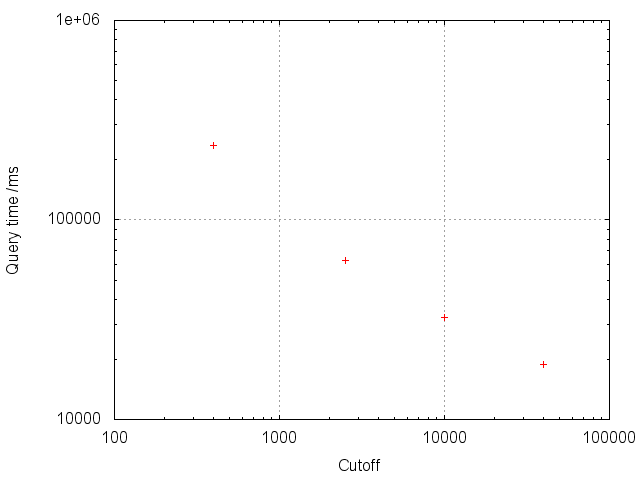
\includegraphics[width=0.80\textwidth]{graph.png}
\end{figure}

As is apparent from the above results, for the queries tested using ForkJoin is the slowest.  This is probably due to very high costs associated with managing many threads.  This claim can be supported by the improved performance as the sequential cutoff becomes larger, and the algorithm is threaded less and becomes more like the sequential variant.  Nonetheless, it is an unexpected result which warrants closer inspection in the future.

On the other hand, file input benefitted greatly for multithreading.  In the benchmark, reading three times as much data took less than twice as long as the single-file sequential case.  This is expected because the bottleneck in this process is string tokenisation and parsing.

The preprocessing for cumulative sums was remarkably fast.  Given that it took 12ms, with na\"ive sequential queries typically taking 0.3ms and preprocessed queries being negligibly quick, only around 40 queries are needed to make this preprocessing the optimal solution.

\section{Conclusions}

In the context of this assignment, parallelisation is not beneficial for queries, although perhaps it would be when dealing with much larger data sets.  The best solution found is a constant-time algorithm using precomputed cumulative sums.

\end{document}
